\documentclass[aspectratio=169]{beamer}
\usetheme{Madrid}
\usepackage[utf8]{inputenc}
\usepackage[T1]{fontenc}
\usepackage{tikz}
\usepackage{amssymb}
\usepackage{graphicx}
\setbeamertemplate{navigation symbols}{}
\setbeamercolor{title}{fg=white,bg=orange!85!red}
\setbeamercolor{frametitle}{fg=white,bg=orange!85!red}
\setbeamercolor{block title}{bg=orange!85!red!20,fg=black}
\setbeamercolor{block body}{bg=orange!85!red!8,fg=black}
\setbeamercolor{item}{fg=orange!85!red}
\setbeamercolor{itemize item}{fg=orange!85!red}
\setbeamertemplate{itemize item}[triangle]

\title{Block Arcade 3 — Events}
\subtitle{Keys are events — the stage reacts to what the player presses}
\author{ByteForge --- Grade 7 --- Game Maker}
\date{}

\begin{document}

\begin{frame}
    \titlepage
\end{frame}

\begin{frame}{Today's Plan}
    \begin{itemize}
        \item Press to Move
        \item Jump on Space
        \item[$\bigstar$] BOSS --- Full Control
    \end{itemize}
\end{frame}

\begin{frame}{Checking a key is a question, asked every frame}
    \large
    \begin{itemize}
        \item Placed inside "on every frame", a key check is asked 60 times a second
        \item That's what makes a held-down key feel like smooth movement.
    \end{itemize}
\end{frame}


\begin{frame}{Any key can trigger any action}
    \large
    \begin{itemize}
        \item Space isn't special
        \item It's just another key. What makes it feel like a "jump" is purely what you put inside the if.
    \end{itemize}
\end{frame}


\begin{frame}{BOSS — four keys, four directions}
    \large
    \begin{itemize}
        \item Each arrow key gets its OWN separate if
        \item Pressing two at once genuinely moves the sprite diagonally, for free.
    \end{itemize}

    \begin{center}
    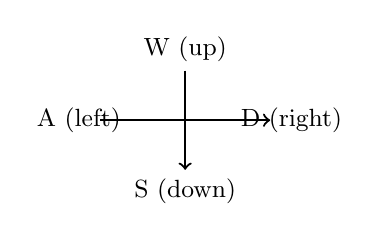
\begin{tikzpicture}[scale=0.9]

        \node at (0,0) {\small W (up)};
        \node at (0,-2) {\small S (down)};
        \node at (-1.5,-1) {\small A (left)};
        \node at (1.5,-1) {\small D (right)};
        \draw[->, thick] (0,-0.3) -- (0,-1.7);
        \draw[->, thick] (-1.2,-1) -- (1.2,-1);
        \node at (0,-1) {\small +};
    \end{tikzpicture}
    \end{center}
\end{frame}

\begin{frame}{Real-World Examples}
    \large
    \begin{itemize}
        \item A car's cruise control constantly re-checking your foot on the brake, or a lift constantly checking if a floor button is pressed
        \item Both are "ask the same question every moment", not a one-time check. Minecraft's own WASD + Space controls are literally this chapter's pattern
        \item Each key its own independent check, which is exactly why you can strafe (A/D) while jumping (Space) at the same time.
    \end{itemize}
\end{frame}


\begin{frame}{Image}
    \begin{center}
    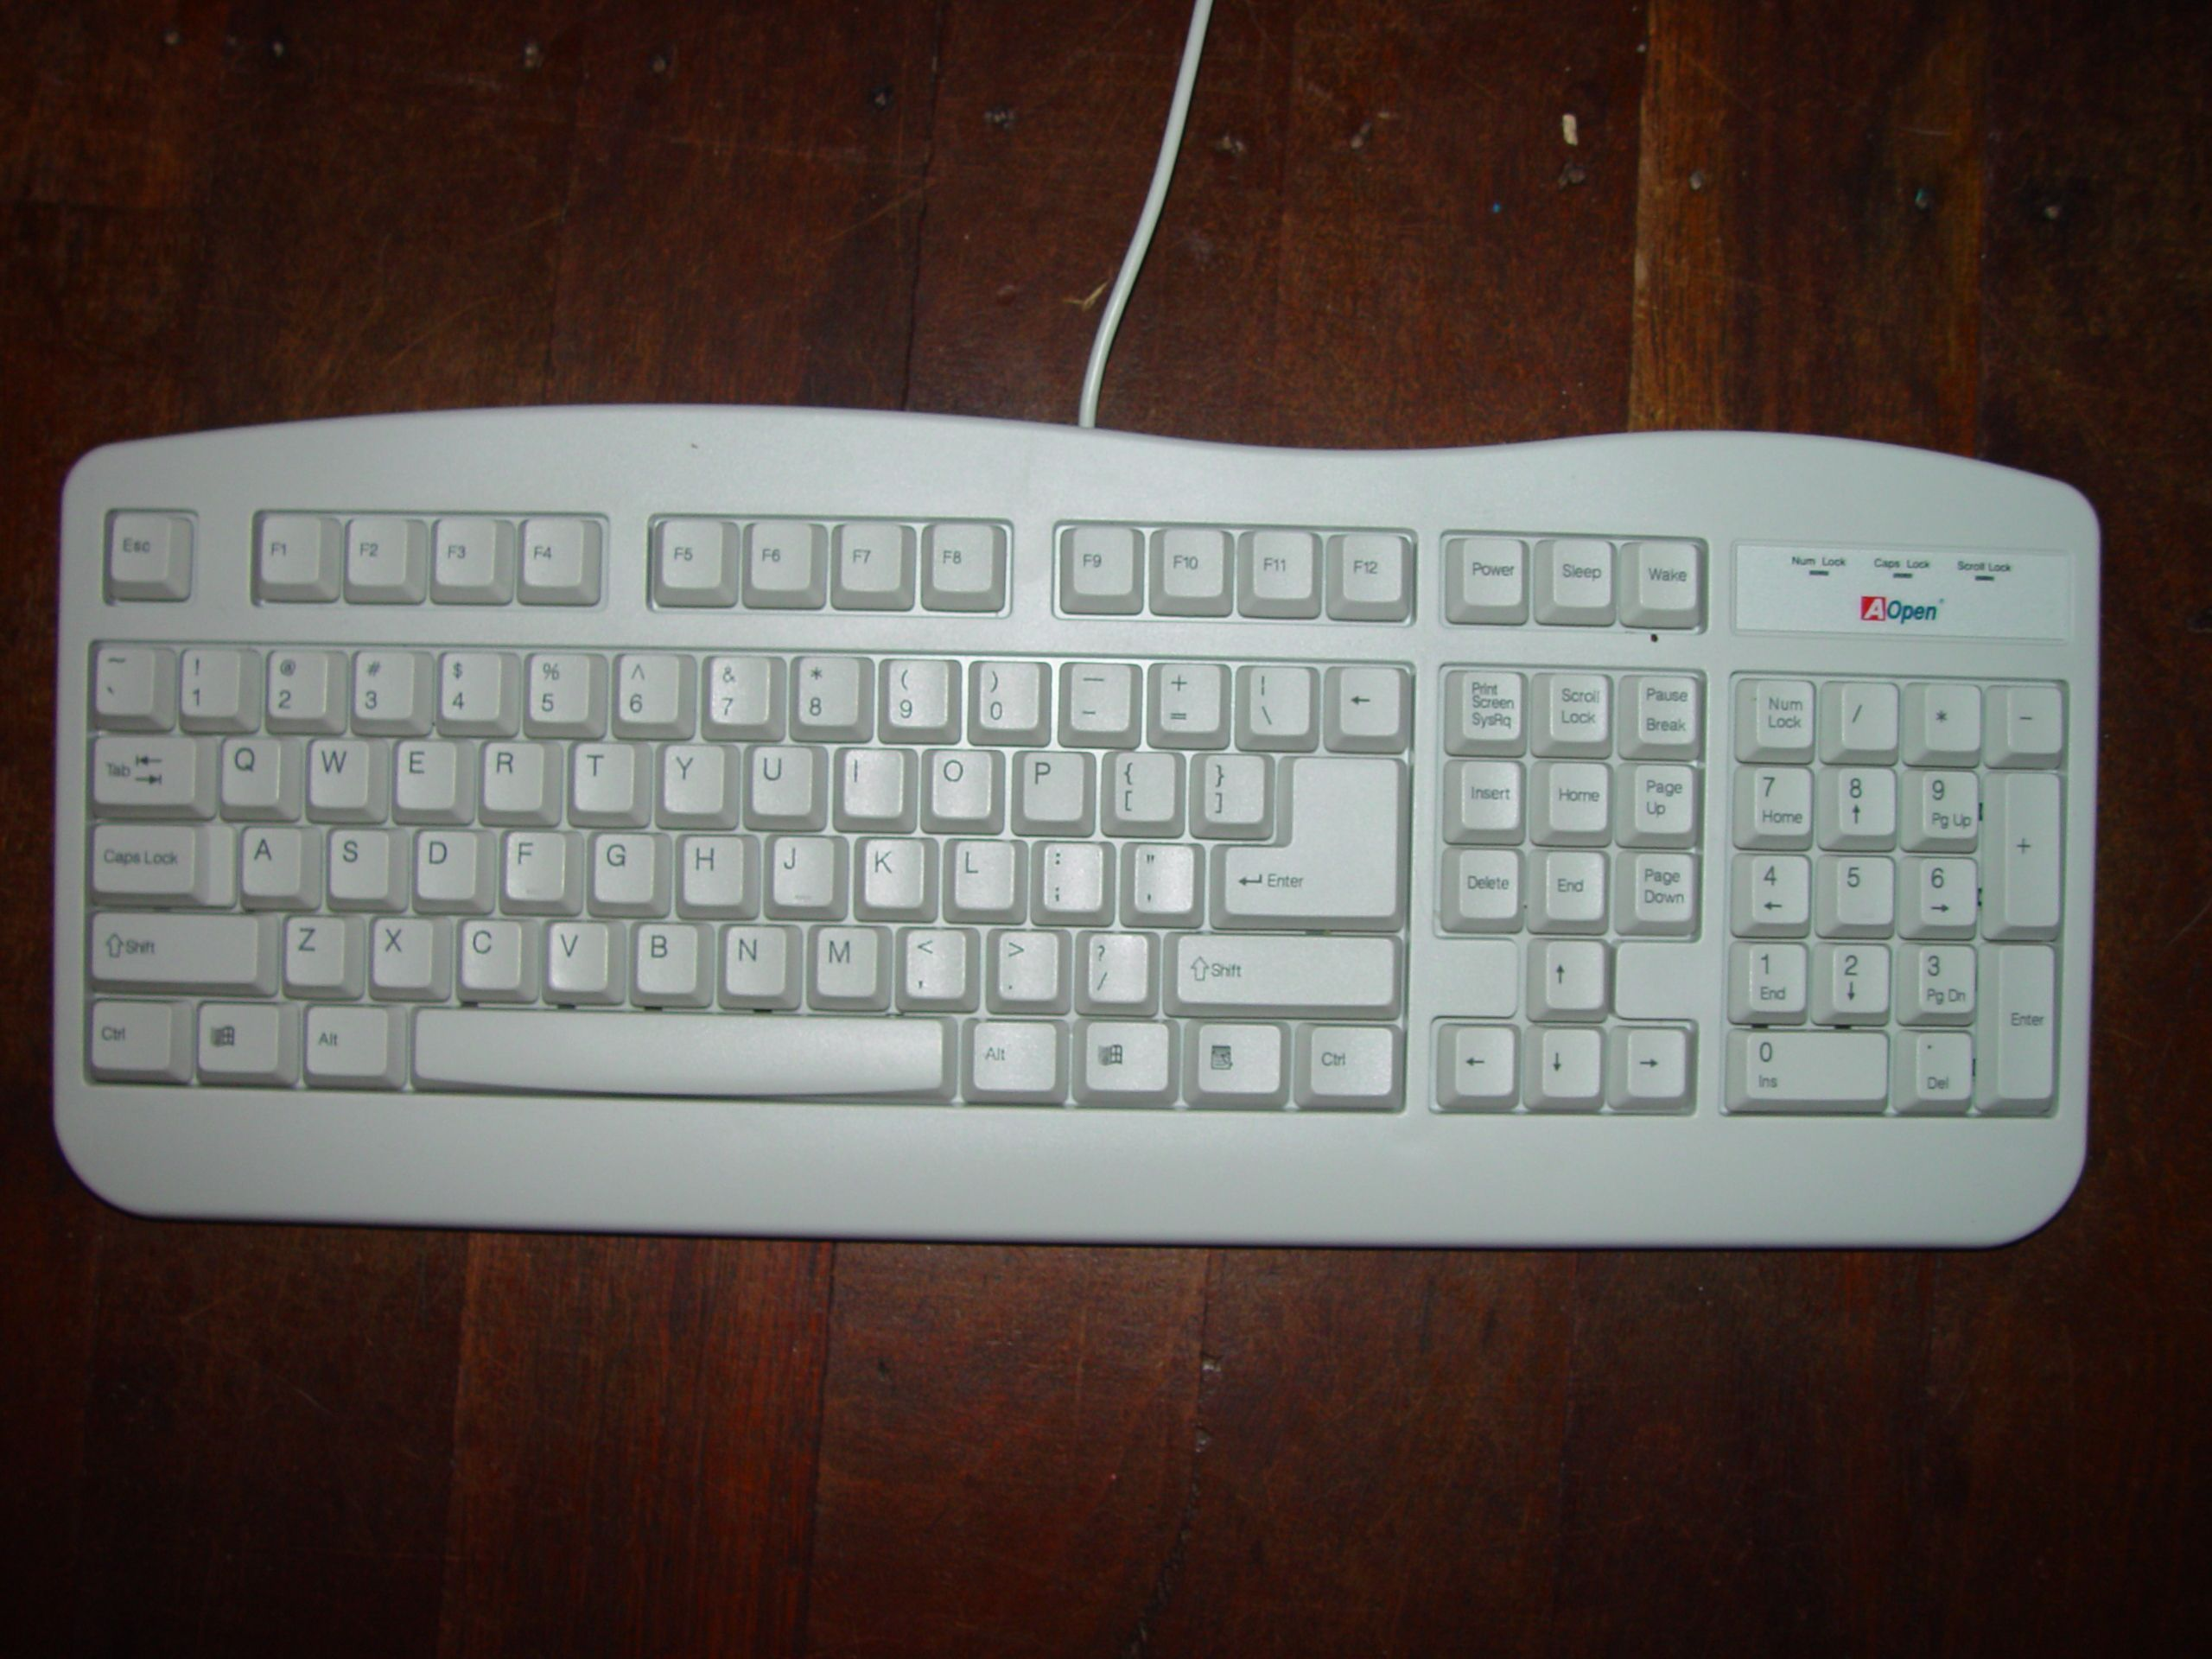
\includegraphics[width=0.5\textwidth]{images/keyboard.jpg}

    \large Every 'key pressed?' check this chapter teaches is a real key on a real board like this.

    \small Computer keyboard, public domain, via Wikimedia Commons
    \end{center}
\end{frame}

\begin{frame}{Let Them Discover}
    \Large
    Try holding two arrow keys at once in any real game (or your phone's on-screen d-pad), or W+Space in Minecraft. Does the character move diagonally / jump-forward? What would the code need to allow that — one if, or two separate ifs?
\end{frame}

\begin{frame}{Your Turn}
    \Large
    Open the student map, find \textbf{Block Arcade 3 — Events}, and work through it
    hands-on --- everything you just saw, they now do themselves.
\end{frame}

\end{document}
